\documentclass[landscape]{slides}
%\usepackage{lscape}
\usepackage{color,graphicx}
\usepackage[colormath,coloremph,colorhighlight,display]{texpower}
%\usepackage[colormath,coloremph,colorhighlight]{texpower}
\usepackage[scaleupmath,scaleuptt]{tpslifonts}
\usepackage{fixseminar}
\pagestyle{empty}
\usepackage{amsmath,amsfonts,amssymb}
\usepackage{fancyvrb}

\newcommand{\xbar}{\bar{X}}
\newcommand{\ybar}{\bar{Y}}
\newcommand{\thetab}{\bar{\theta}}
\newcommand{\thetalb}{\underset{\bar{}}{\theta}}
\newcommand{\nX}{X_1,X_2,\ldots,X_n}
\newcommand{\nx}{x_1,x_2,\ldots,x_n}
\newcommand{\nY}{Y_1,Y_2,\ldots,Y_n}
\newcommand{\ny}{y_1,y_2,\ldots,y_n}


\newcommand{\slidetitle}[1]{\begin{center}{\large\bf \color{red} #1}\end{center}}

\newcommand{\ddt}{{\textstyle\frac{\rm d}{{\rm d}t}}}
\renewcommand{\d}{\mbox{d}}
\newcommand{\N}{{\mathcal{N}}}
\newcommand{\IG}{{\mathcal{IG}}}
\newcommand{\DP}{{\mathcal{DP}}}
\newcommand{\Ga}{{\mathcal{G}a}}
\newcommand{\R}{{\mathbb{R}}}
\renewcommand{\P}{{\mathbb{P}}}
\newcommand{\E}{{\mathbb{E}}}
\newcommand{\I}[1]{{\mathbb{I}}_{\{#1\}}}
\renewcommand{\bold}[1]{\mbox{\boldmath$#1$}}

\replacecolor{emcolor}{red}



\newcommand{\heading}[1]{%
  \begin{center}
    \large\bf \color{red}
%    \shadowbox{#1}%
        #1
  \end{center}
  \vspace{1ex minus 1ex}}
\begin{document}

%%%%%%%%%%%%%%%%%%%%%%%%%%%%%%%%%%%%%%%%%%%%%%%%%%%%%%%%%%%%
\begin{slide}
\heading{Outline}
\vskip 1.0cm
{\em 1)} Linear models -- simple linear regression

{\em 2)} Model formulation

%{\em 3)} Linear least squares

%{\em 4)} Maximum likelihood estimators
\end{slide}
%%%%%%%%%%%%%%%%%%%%%%%%%%%%%%%%%%%%%%%%%%%%%%%%%%%%%%%%%%%%




\begin{slide}
	\heading{Simple Linear Regression}
	{\bf Mitsubishi Example:}
	
	Ingrid wants to buy second-hand Mitsubishi Sigmas for her business. To estimate the cost, her team collects data on the age and price of 39 cars.
	
	  \begin{minipage}{0.55\textwidth}
		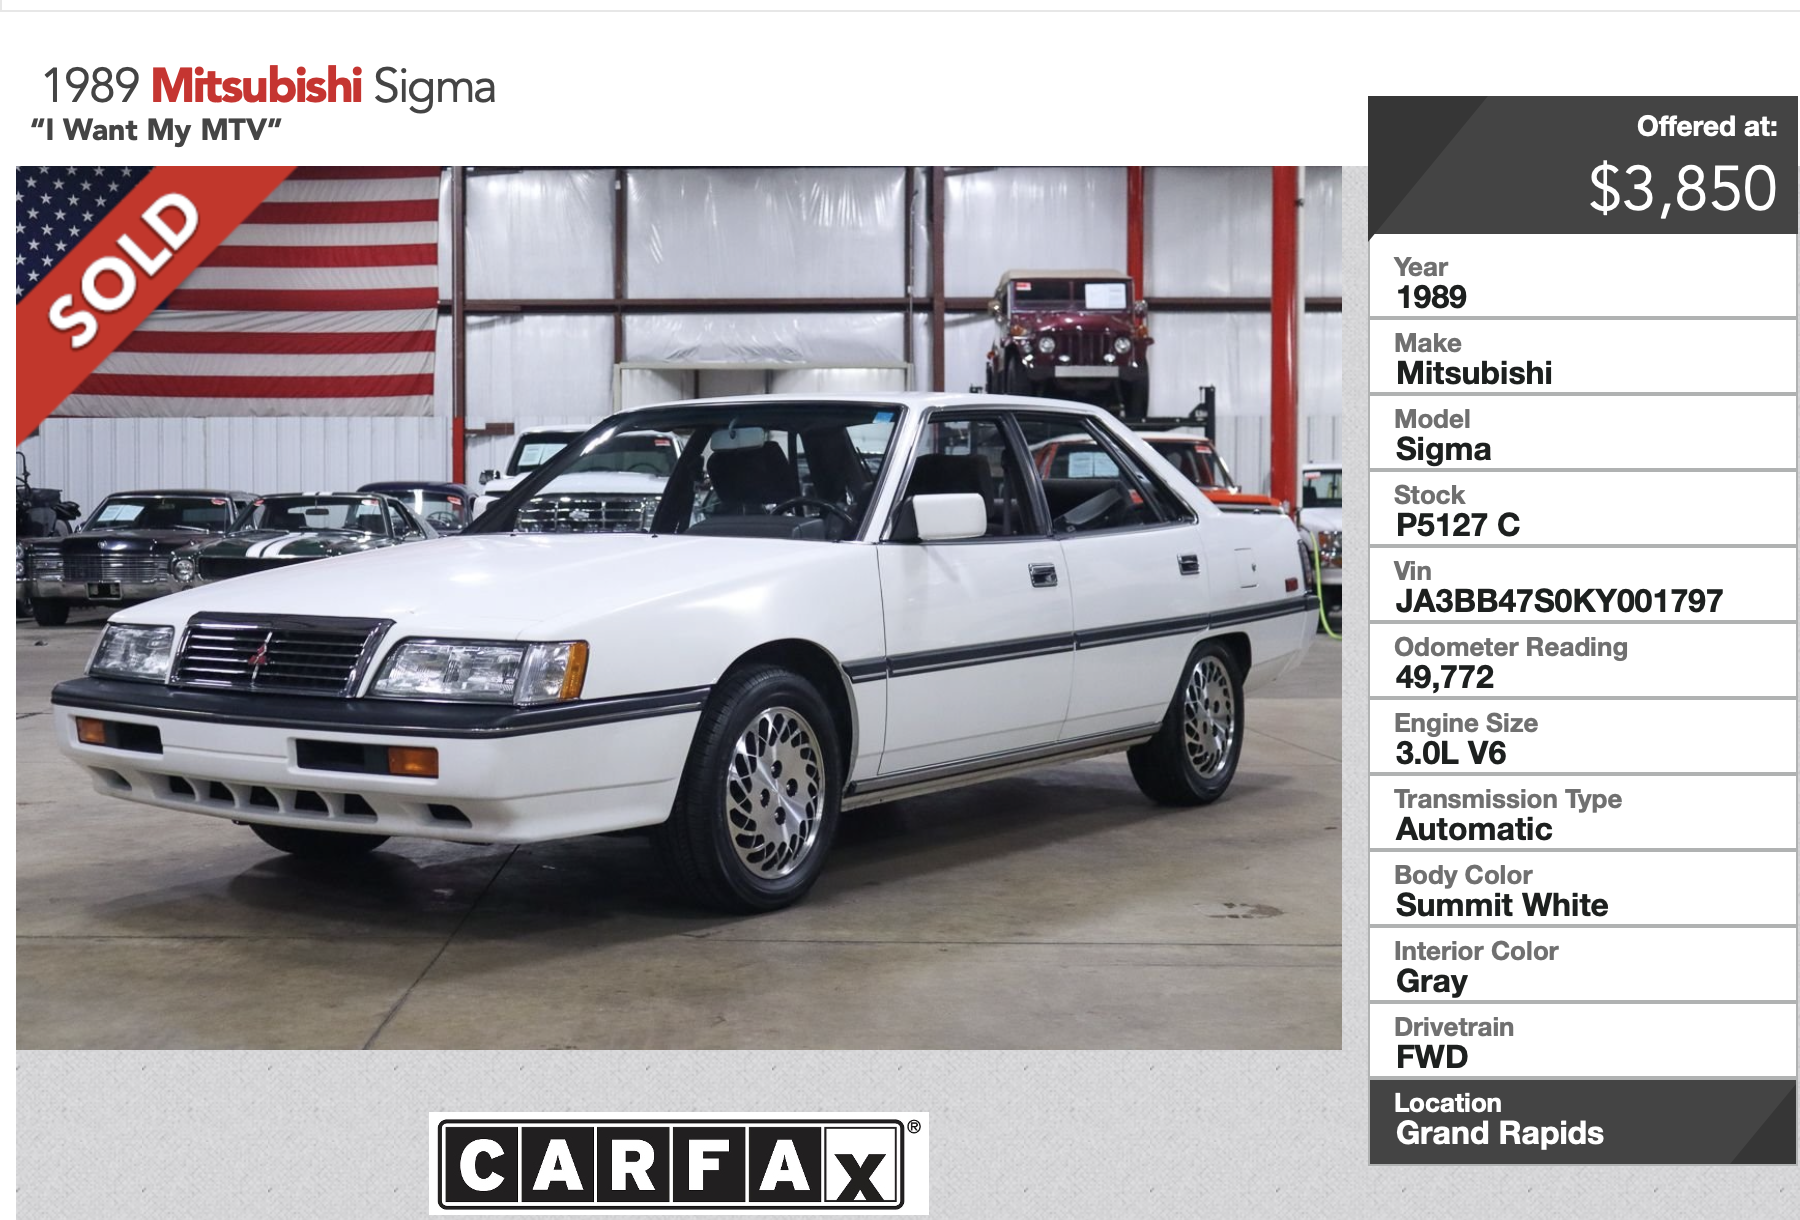
\includegraphics[width=\textwidth]{car.png}
	\end{minipage}%
	\begin{minipage}{0.35\textwidth}
		\textcolor{blue}{  Can she use this data to predict how much she'll pay for the cars?}
	\end{minipage}
	
\end{slide}


\begin{slide}
\heading{Mitsubishi Example}
%
\textcolor{magenta}{Download the dataset ({\tt mitsub.txt}) and load it in RStudio.}

A first step might be to look at some summary statistics:
%
{\small
\begin{verbatim}
> summary(mitsub)
      age            price     
 Min.   : 6.00   Min.   : 450  
 1st Qu.:10.00   1st Qu.:2850  
 Median :12.00   Median :3500  
 Mean   :11.79   Mean   :3625  
 3rd Qu.:14.00   3rd Qu.:4350  
 Max.   :15.00   Max.   :8999  
\end{verbatim}
}

Some standard statistical calculations allow Ingrid to predict with 95\%
certainty that a randomly chosen second hand sigma will cost between
\$668 and \$6625. 
\textcolor{magenta}{Use the {\tt quantile} function to find these values }
\end{slide}


\begin{slide}
	\heading{Mitsubishi Example}
	
	\begin{itemize}
		\item Ingrid needs to estimate the cost of building her fleet.
		\item Current prediction range is too wide to be useful.
		
		\item Improvement idea:
		\begin{itemize}
			\item Use additional data, like car age, to improve predictions.
			\item {\tt age} and {\tt price} are likely correlated.
		\end{itemize}
		
		\item Scatterplot of {\tt price} vs {\tt age} (below) shows prices decrease as cars age. % \textcolor{magenta}{Q: Write the code to create this scatterplot.}
	\end{itemize}
	
\end{slide}


\begin{slide}
\heading{Mitsubishi Example}

\begin{center}
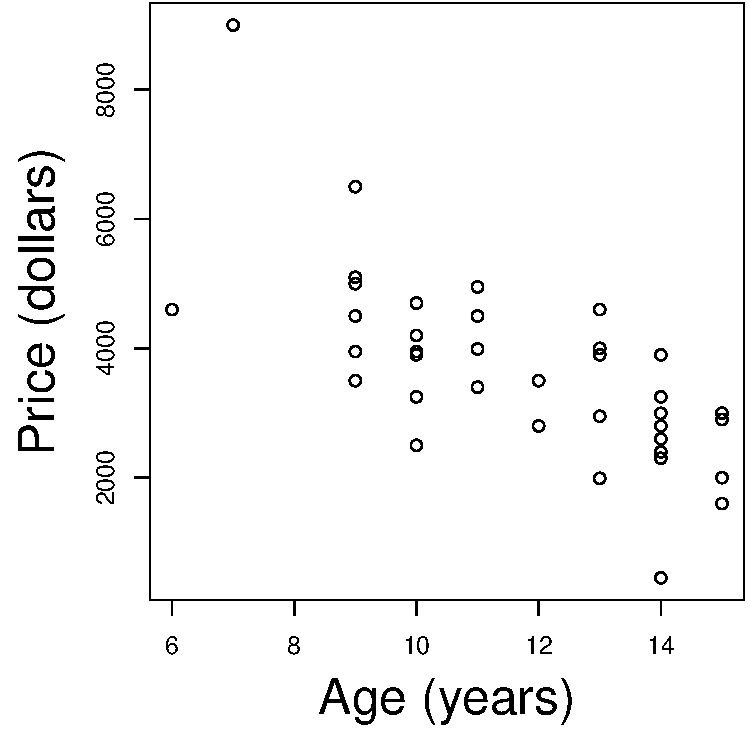
\includegraphics{figures/7-LinearModels-Figures/ageprice.pdf}
\end{center}
\end{slide}


\begin{slide}
	\heading{Mitsubishi Example}
	
	\begin{itemize}
		\item Goal: Predict the price of a 10-year-old car.
		\item Average price for 10-year-old cars: \$3750.
		\item Average price for 14-year-old cars: \$2587. \textcolor{magenta}{Find these values using R.}
		
		\item Repeat for different ages to get average prices at various ages.
		\item The plot below shows how average price changes with age.
		
%		\item \textcolor{magenta}{Q: Write the R code to create this plot.}
	\end{itemize}
	
\end{slide}

\begin{slide}
\heading{Mitsubishi Example}

\begin{center}
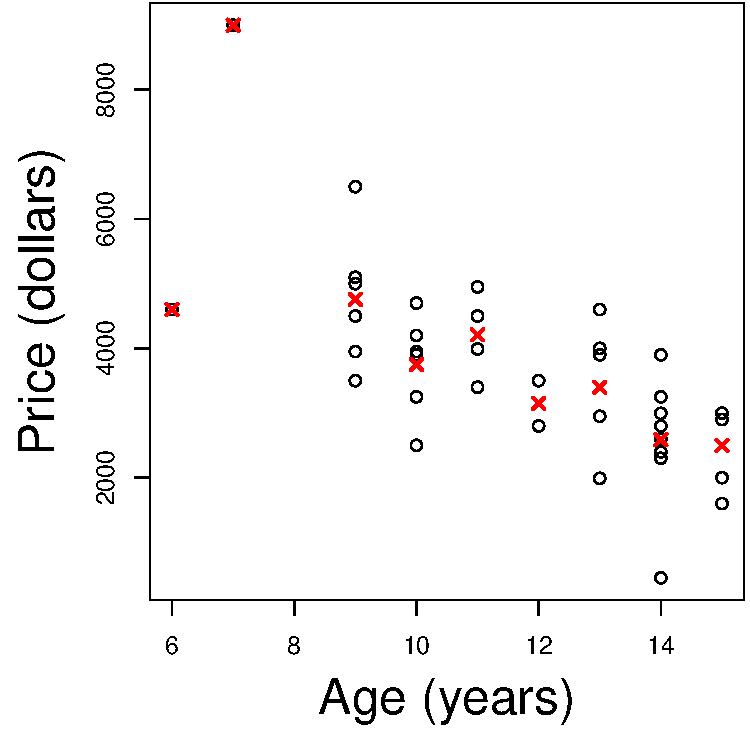
\includegraphics{figures/7-LinearModels-Figures/agepricex.pdf}
\end{center}
\end{slide}

\begin{slide}
	\heading{Mitsubishi Example}

	\begin{itemize}
		\item A finer strip leads to a “regression curve”: the mean price for each age.\vspace{-1em}
		\item We could use the prices of 10-year-old cars to create a new prediction interval.\vspace{-1em}
		\item However, there are only 5 cars aged 10, so accuracy is limited.\vspace{-1em}
		\item For other ages, the data is even sparser:
		\begin{itemize}
			\item Only 2 cars are 12 years old.
			\item No cars are 8 years old in the sample.
		\end{itemize}\vspace{-1em}
		\item How can we use this sparse data to predict prices for these ages?
	\end{itemize}
	
\end{slide}

\begin{slide}
	\heading{Mitsubishi Example}
	
	\begin{itemize}
		\item To predict prices, we model the  "regression curve".
		\item The plot suggests the curve is roughly  "linear".
		\item We can assume a  "simple linear regression model" to predict price based on age.
		

		\item The fitted model is:
		$$\hat{\mbox{price}} = 8452 - 409 \; {\tt age}$$
	\end{itemize}
	
\end{slide}

\begin{slide}
	\begin{center}
		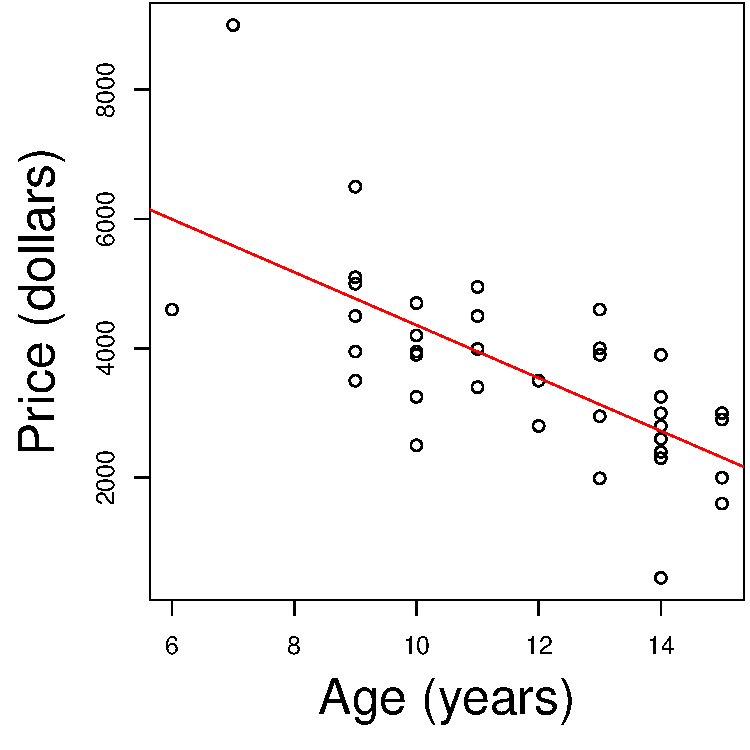
\includegraphics[width=0.5\textwidth]{figures/7-LinearModels-Figures/mitsub_reg.pdf}
	\end{center}
	
\end{slide}



\begin{slide}
\heading{Model formulation}
\begin{itemize}
\item In the Mitsubishi example, we say that {\tt age} is a \textcolor{blue}{\bf predictor} for 
{\tt price}. The variable {\tt age} is called the \textcolor{blue}{\bf predictor variable} and
{\tt price} is the \textcolor{blue}{\bf response variable}.

\item The usual generic notation for simple regression is
$$x=\mbox{ predictor variable}$$
$$y=\mbox{ response variable}$$

\item The prediction equation is
%
$$\hat{y}=\beta_0+\beta_1 x$$
\end{itemize}
\end{slide}
\begin{slide}
\heading{Model formulation}
\begin{itemize}

\item Therefore, if $y$ is any particular observation with corresponding $x$-value equal to 
$x$ then we can write 
$$y=\beta_0+\beta_1 x+\epsilon$$
where the {\it error } $\epsilon$ is given by
$$\epsilon=y-\hat{y}=y-(\beta_0+\beta_1 x)$$
		\item The \textbf{error term} ($\epsilon$) represents the difference between what we predict ($\hat{y}$) and what we actually observe ($y$).
\end{itemize}
\end{slide}


\begin{slide}
	\begin{center}
		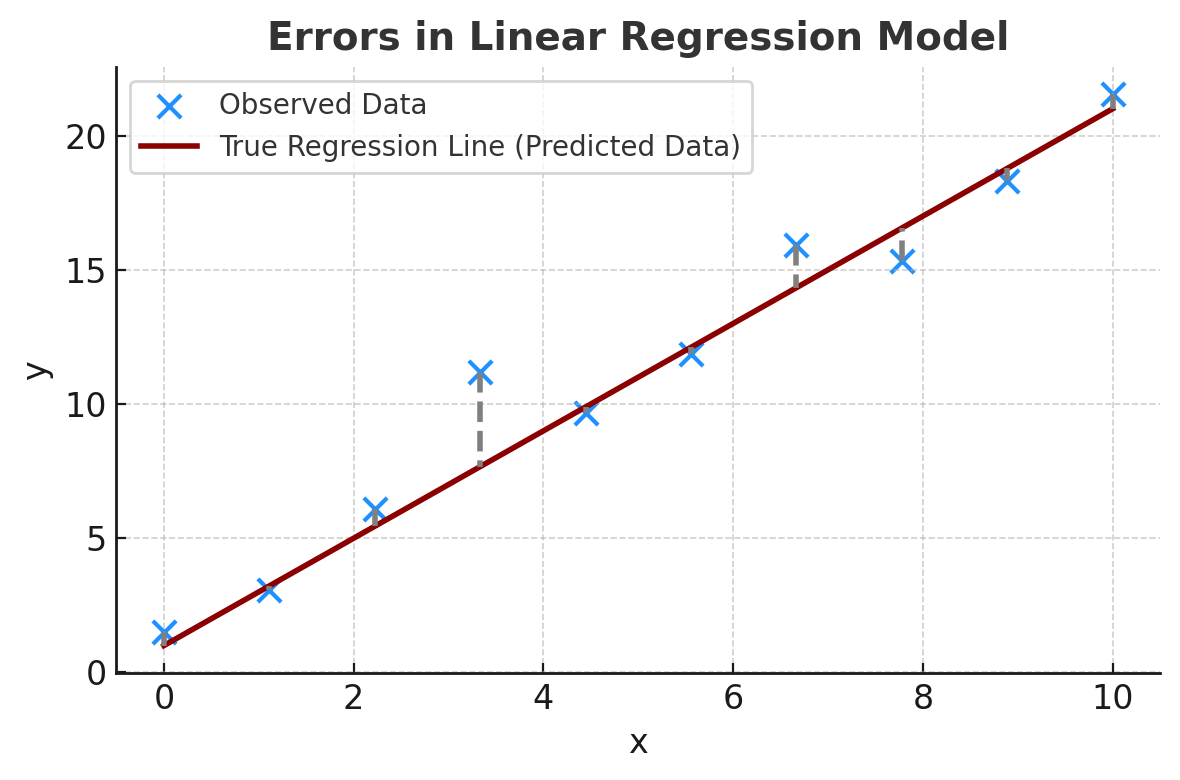
\includegraphics[width=1\textwidth]{errors.png}
	\end{center}
	
\end{slide}

\begin{slide}
	\heading{Understanding the Error Terms}
	\begin{itemize}

		
		\item The first assumption we make is:
		$$E(\epsilon) = 0$$
		This means that on average, the errors cancel out. Sometimes we predict too high, sometimes too low, but overall the average error is zero.
	
		\item Finally, we assume the errors follow a \textbf{normal distribution}:
		$$\epsilon \sim N(0, \sigma^2)$$
		This means that most errors are small (close to zero), and bigger errors are less likely. The error distribution is symmetric around 0, with the spread determined by $\sigma^2$.

	\item The \textbf{variance of the error} tells us how spread out the errors are:
$$Var(\epsilon) = \sigma^2$$
This tells us that the errors vary by a certain amount (denoted as $\sigma^2$). It gives an idea of how far off our predictions could be from reality.

	\end{itemize}
\end{slide}

\begin{slide}
	\heading{What is a Normal Distribution?}
	\begin{itemize}
		\item The \textbf{normal distribution} is a bell-shaped curve where most values (in our case, errors) are close to the center (0), and fewer values are far away from the center.
		
		\item This curve is symmetric, meaning that errors are equally likely to be positive or negative.
		
		\item For our model:
		$$\epsilon \sim N(0, \sigma^2)$$
		This means the average error is 0, and the spread (how far errors go from 0) is determined by $\sigma^2$.
		
		\item Here is what the normal distribution looks like:
		
		\begin{center}
			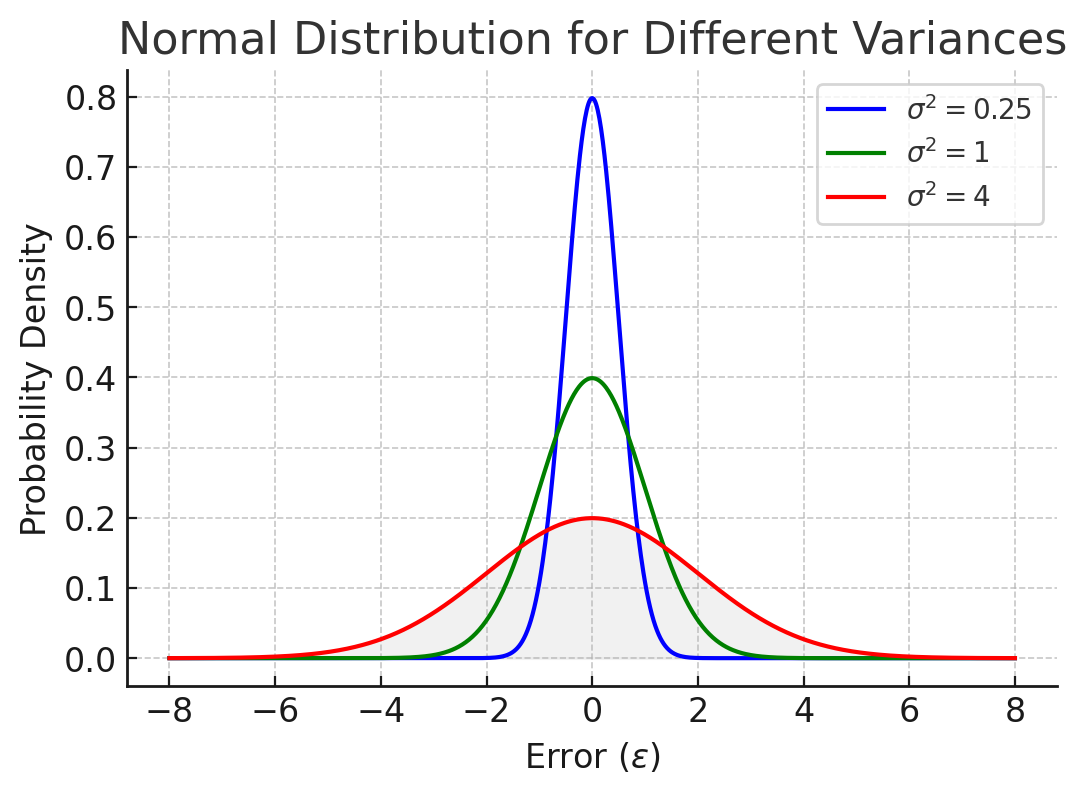
\includegraphics[width=0.5\textwidth]{normal_distribution.png}
		\end{center}
		\item Most errors are close to zero, but sometimes we can have larger errors, though these are less likely.
	\end{itemize}
\end{slide}



\begin{slide}
\heading{Model formulation}
\begin{itemize}

\item Thus we can write the simple linear regression model as
$$y=\beta_0+\beta_1 x+\epsilon, \quad \epsilon \sim N(0,\sigma^2).$$

\item Suppose we have $n$ observations, \\
$(x_1,y_1),\ldots,(x_n,y_n)$ from this model, then
$$y_i=\beta_0+\beta_1 x_i+\epsilon_i, i=1,\ldots, n$$
%
\item We assume further that the observations are collected independently of each other so that
the $\epsilon_i$ are independent. This means that a knowledge of one of the $e_i$ does not tell
us anything about the value of the other $e_i$s

\end{itemize}
\end{slide}
%\begin{slide}
%\heading{Linear Least Squares}
%5\begin{itemize}
%\item In order to fit a straight line to a plot of points
%$(x_i,y_i)$, where $i=1,\ldots,n$, the slope and intercept of the
%line 
%$$y =\beta_0+\beta_1x$$
%must be found from the data in some manner
%
%\item In order to fit a $p$-th order polynomial, $p+1$ coefficients must
%be determined
%
%\item Other functional forms besides linear and polynomial ones may be fit to 
%data, and in order to do so, parameters associated with those forms must be
%determined
%
%\end{itemize}
%\end{slide}
%\begin{slide}
%\heading{Linear Least Squares}
%\begin{itemize}
%\item The most common method for determining the parameters in curve-fitting
%problems is the method of least squares

%\item The idea is to minimize the sum of squared deviations of the predicted,
%or {\it fitted} values, (given by the curve) from the actual observations.

%\item Applying the method of {\bf least squares}, we choose the slope and
%intercept of the straight line to minimize
%$$S(\beta_0,\beta_1)=\sum_{i=1}^n (y_i-\beta_0-\beta_1x_i)^2$$
%
%\item Note that $\beta_0$ and $\beta_1$ are chosen to minimize the sum of squared
%vertical deviations, or prediction errors
%\end{itemize}
%\end{slide}
%\begin{slide}
%\heading{Linear Least Squares}
%\begin{itemize}

%\item To find $\beta_0$ and $\beta_1$, we calculate
%$$\frac{\partial S}{\partial\beta_0}=-2\sum_{i=1}^n(y_i-\beta_0-\beta_1x_i)$$
%$$\frac{\partial S}{\partial\beta_1}=-2\sum_{i=1}^nx_i(y_i-\beta_0-\beta_1x_i)$$

%\item Setting these partial derivatives equal to zero, we have that the minimizers
%$\hat{\beta}_0$ and $\hat{\beta}_1$ satisfy
%$$\sum_{i=1}^ny_i=n\hat{\beta}_0+\hat{\beta}_1\sum_{i=1}^nx_i$$
%$$\sum_{i=1}^nx_iy_i=\hat{\beta}_0\sum_{i=1}^nx_i+\hat{\beta}_1\sum_{i=1}^nx_i^2$$

%\item Solving for $\hat{\beta}_0$ and $\hat{\beta}_1$ , we obtain
%$$\hat{\beta}_0=\frac{(\sum_{i=1}^nx_i^2)(\sum_{i=1}^ny_i)-(\sum_{i=1}^nx_i)(\sum_{i=1}^nx_iy_i)}{n\sum_{i=1}^nx_i^2-(\sum_{i=1}^nx_i)^2}$$

%$$\hat{\beta}_1=\frac{n\sum_{i=1}^nx_iy_i-(\sum_{i=1}^nx_i)(\sum_{i=1}^ny_i)}{n\sum_{i=1}^nx_i^2-(\sum_{i=1}^nx_i)^2}$$

%\end{itemize}
%\end{slide}
%\begin{slide}
%\heading{Linear Least Squares}
%\begin{itemize}

%\item Functional forms more complicated than straight lines are often fit to data,
%for example, when there are more than one predictor variables available, we may
%fit a line of the form
%$$y\approx \beta_0+\beta_1x_1+\beta_2x_2+\beta_3x_3$$
%where $\beta_i$ could be estimated from data
%\end{itemize}
%\end{slide}
%\begin{slide}
%\heading{Linear Least Squares}
%\begin{itemize}
%

%\item Or we may be able to fit functions of the following form to decay curves
%$$f(t)=Ae^{-\alpha t}+Be^{-\beta t}$$
%where the function $f$ is linear in the parameters $A$ and $B$ and nonlinear
%in the parameters $\alpha$ and $\beta$,  
%from data of the form $(y_i,t_i), i=1,\ldots,n$

%\item When the function to be fitted is linear in the unknown parameters, the 
%minimisation is relatively straightforward, since calculating partial derivatives
%and setting them equal to zero produces a set of simultaneous linear equations
%that can be solved in closed form. This special case is known as {\bf linear
%east squares}
%\end{itemize}
%\end{slide}

\begin{slide}
\heading{Mitsubishi Example:}

For the Mitsubishi price/age data, using the R commands 

\begin{Verbatim}[commandchars=\\\{\}]
> mitsub.lm <- lm(price ~ age, data = mitsub)
> summary(mitsub.lm)
\end{Verbatim}


%


gives that the estimates of the coefficients are
$$\hat{\beta}_0=8451.591 \quad \hat{\beta}_1=-409.2175$$

and the residual variance is
$$\hat{\sigma}^2=1045^2$$

\end{slide}

\begin{slide}
	
	\begin{center}
		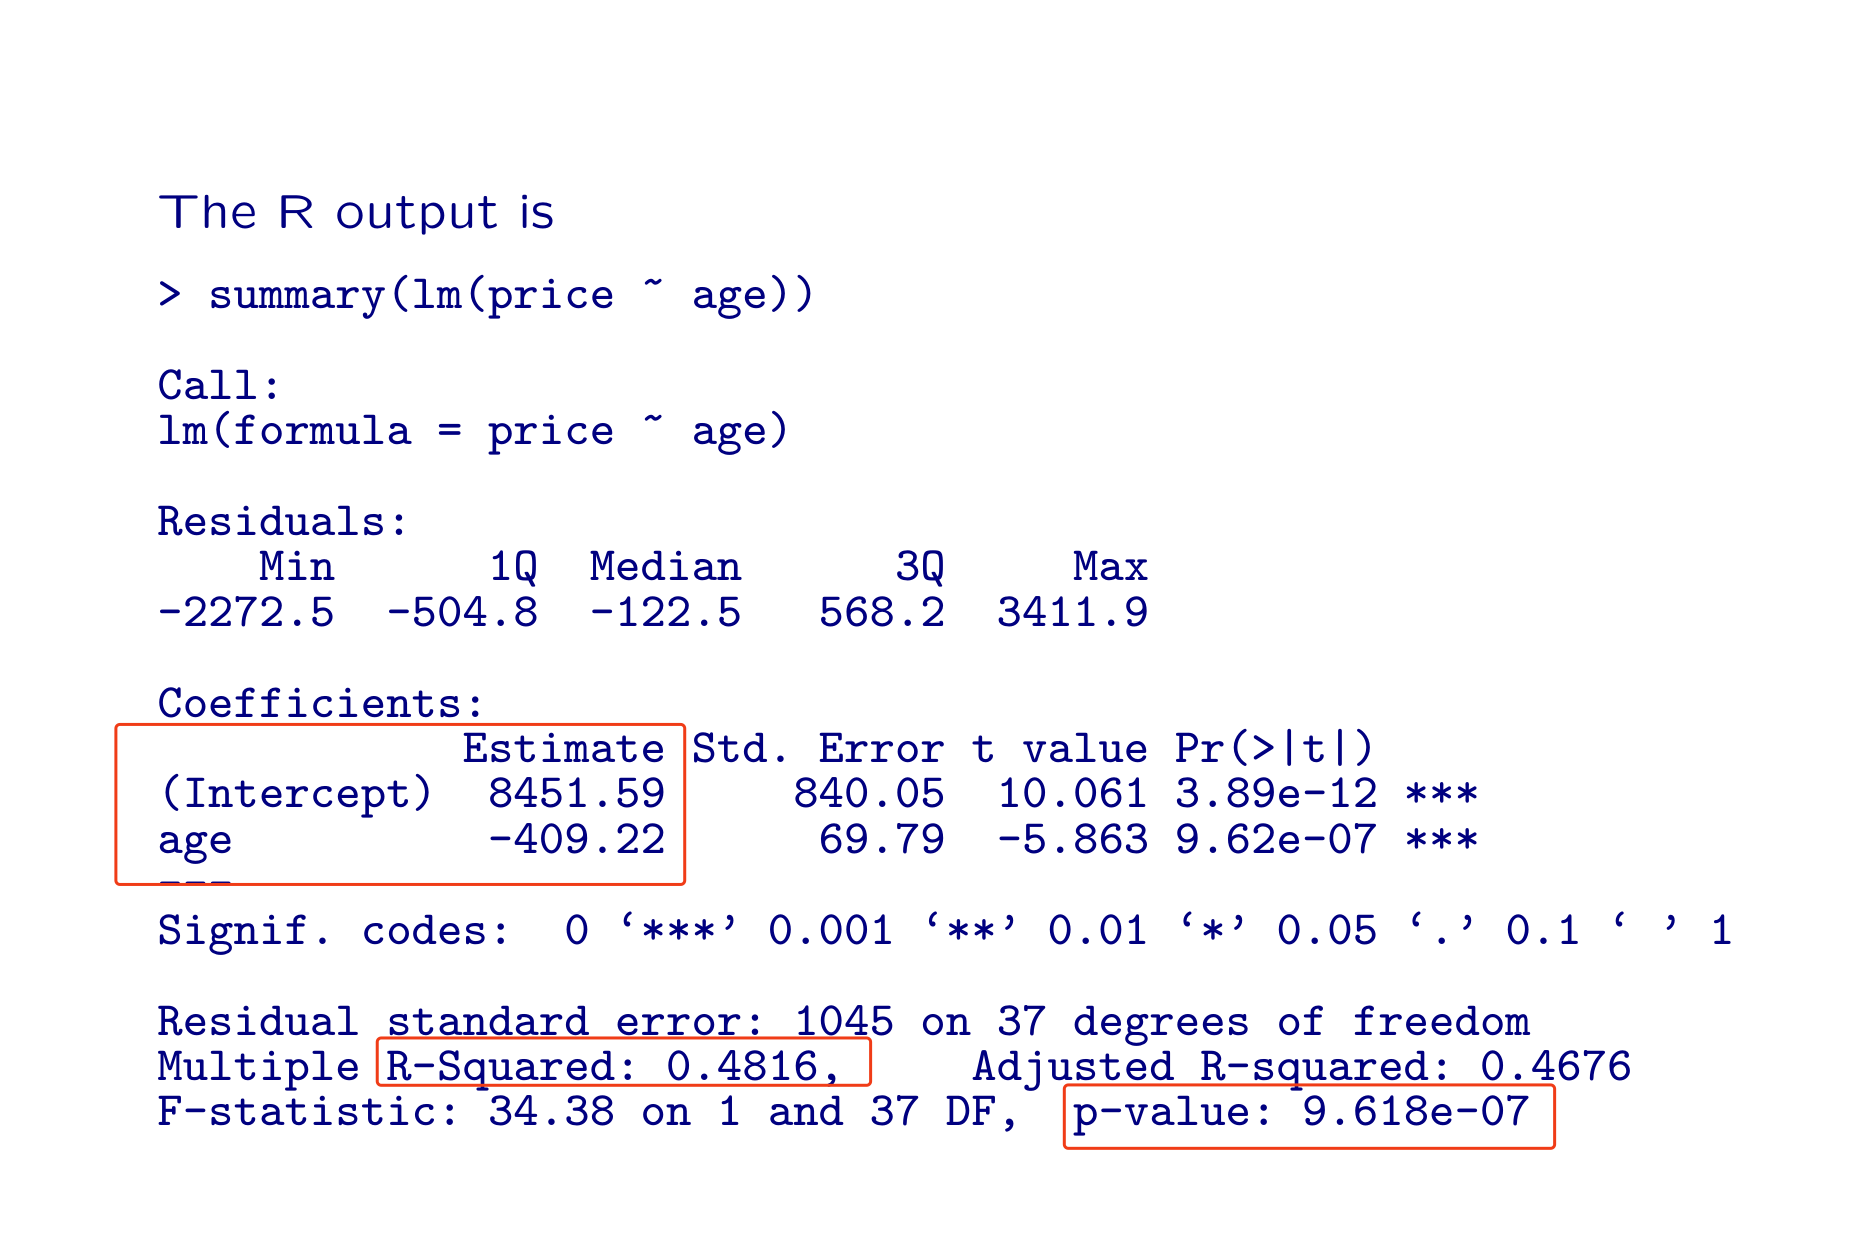
\includegraphics[width=1\textwidth]{output.png}
	\end{center}
\end{slide}


\begin{slide}
	\heading{Understanding Linear Regression Results}
	\begin{itemize}
		\item \textbf{Goal:} We are trying to predict the price of something based on its age. The output shows the results of this prediction.
		
		\item \textbf{Intercept (8451.59):} This means that if the age is 0, the predicted price is \$8451.59. It's the starting point of our prediction line.
		
		\item \textbf{Slope (-409.22):} For every 1 year increase in age, the price decreases by \$409.22. This tells us that older things are worth less.
		
	%	\item \textbf{Residuals:} These numbers show how far off our predictions are from the actual prices. Some predictions are too high, some too low, but overall, they average out.
		
		\item \textbf{R-Squared (0.4816):} About 48\% of the price changes can be explained by the age. This is how well our model fits the data.
		
		\item \textbf{p-value (9.62e-07):} This number tells us if age is important for predicting the price. Since it's very small, we can say age is a very important factor.
		
	\end{itemize}
\end{slide}


\begin{slide}
\heading{Mitsubishi Example:}

Hence the fitted line is 
$$\hat{\mbox{price}}=8451.59-409.22 \mbox{ age}.$$

The estimated price of new Mitsubishi Sigma cars ({\tt age =0}) is \$8451.59

The estimated depreciation rate of Mitsubishi Sigma cars is \$409.22 per year

\end{slide}
 

\begin{slide}
	\heading{Mitsubishi Example:}
	 
	
	The standard error of the intercept, $s_{\hat{\beta}_0}=840.05$. A 95\% confidence
	interval for the intercept, $\beta_0$ based on the $t$ distribution with 37 df is
	$$\hat{\beta}_0\pm t_{37}(0.025)s_{\hat{\beta}_0} \Longrightarrow (6748.897, 10153.10).$$
 
	Similarly, a 95\% confidence interval for the slope $\beta_1$, is
	$$\hat{\beta}_1\pm t_{37}(0.025)s_{\hat{\beta}_1} \Longrightarrow (-550.628, -267.8120).$$
	
	To test the null hypothesis $H_0:\beta_0=0$, we would use the $t$ statistic
	$\hat{\beta}_0/s_{\hat{\beta}_0}=10.061$. The hypothesis would be rejected at significance level
	$\alpha=0.05$, there is strong evidence that the intercept is non-zero.
	
 
	
\end{slide}


\end{document}


